\documentclass{beamer}
\usepackage{amsmath,amssymb,amsthm,array}
\usepackage{bm}
\usepackage{xltxtra}
\usepackage{multirow}
\usepackage{multicol}
\usepackage{listings}
\usepackage{algorithm}
\usepackage{algorithmic}
\usepackage{verbatim}
\usetheme{cambridgeUS}
\usecolortheme{wolverine}
\usefonttheme{serif}
\setmainfont[Mapping=TeX-text]{GFS Neohellenic}
\setbeamertemplate{navigation symbols}{}
\title{Voting with Blind Signatures}
\author{Panagiotis Grontas}
\date{26/03/2014}
\defbeamertemplate*{footline}{shadow theme}
{%
  \leavevmode%
  \hbox{\begin{beamercolorbox}[wd=.5\paperwidth,ht=2.5ex,dp=1.125ex,leftskip=.3cm plus1fil,rightskip=.3cm]{author in head/foot}%
    \usebeamerfont{author in head/foot}\insertframenumber\,/\,\inserttotalframenumber\hfill\insertshortauthor (\insertshortinstitute)
  \end{beamercolorbox}%
  \begin{beamercolorbox}[wd=.5\paperwidth,ht=2.5ex,dp=1.125ex,leftskip=.3cm,rightskip=.3cm plus1fil]{title in head/foot}%
    \usebeamerfont{title in head/foot}\insertshorttitle%
  \end{beamercolorbox}}%
  \vskip0pt%
}
\institute{$\mu\Pi\lambda\forall$  - CoReLab Crypto Group}
\newcommand{\zns}[1]{ \mathbb{Z}_{#1}^* }
\newcommand{\zn}[1]{ \mathbb{Z}_{#1}}
\newcommand{\md}[1]{\quad (mod \, {#1})}
\newcommand{\pret}{Pr{\^e}t {\`a} Voter }
\newcommand{\vc}{ \mathfrak{c} }
\newcommand{\adv}{ \mathcal{A}  }
\newcommand{\mn}{ \mathcal{M}\mathcal{N}   }
\newcommand{\bb}{ \mathcal{B}\mathcal{B}   }
\newcommand{\prv}{ \mathcal{P}  }
\newcommand{\vrf}{ \mathcal{V}  }

\setlength{\columnseprule}{0.4pt}
\begin{document}


\begin{frame}
\titlepage
\end{frame}

\begin{frame}[allowframebreaks]{Blind Signatures}

\begin{block}{Definition}
A set of algorithms $(Blind, Sign, Verify, Unblind)$:
\begin{enumerate}
\item The message $m$ to be signed is blinded using the Blind Algorithm and some randomness. $b=Blind(m,r)$
\item Afterwards it is signed $S_b = Sign(b)$ in a way that the signature is transferred to the original message.
\item The Unblind function is used on the blind signature obtaining: $S_m = Unblind(S_b)$
\item The signature is verified by executing $Verify(S_m)$
\end{enumerate}
\end{block}

\begin{block}{RSA BS}
\begin{enumerate}
\item $b = Blind(m,r) = r^e H(m) \md{n}$
\item $S_b = Sign(b) = r^{ed \md{\phi(n)}} H(M)^d \md{n} = r H(m)^d $
\item $S_m = Unblind(S_b) = S_b \frac{1}{r} = H(m)^d \md{n}$
\item The signature is verified by executing $Verify(S_m) = $ if ${S_m}^{e} = H(m)$ then $True$ else $False$
\end{enumerate}
\end{block}
\end{frame}

\begin{frame}[allowframebreaks]{Blind Signatures and Voting \cite{chaum83blindsign}}

\begin{itemize}
\item The voter submits a blinded version of the ballot along with his registration information. 
\item The voting authority validates the voter data, and if the voter has the right to vote, signs the blinded ballot and returns it to the voter. 
\item The voter validates the signature of the authority and posts the signed ballot \textit{anonymously}. 
\item The authority receives the signed ballots, validates its signature and posts them to a bulletin board for verification. Verification is done through a random pattern that the voter has embedded into the ballot, known only to him.
\end{itemize}

\begin{block}{Properties}
\begin{itemize}
\item Anonymity
\item Individual verifiability
\item The authority knows the intermediate voting results
\item Dispute Resolution: The voter must show its vote $\rightarrow$ Anonymity is lost
\end{itemize}
\end{block}
\end{frame}

\begin{frame}[allowframebreaks]{A Practical Secret Voting Scheme for Large Scale Elections \cite{FOO92}}

\begin{figure}[hbtp]
\centering
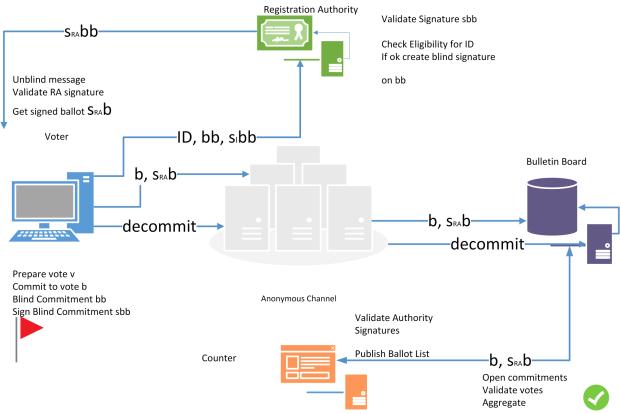
\includegraphics[scale=3]{foo.png} 
\caption{Voting with blind signatures \cite{FOO92}}
\end{figure}

\framebreak

Separate the functions of the authority
\begin{itemize}
\item The registration authority, that knows the voter's identity but not the actual vote 
\item The tallying authority, that knows the vote but not the identity
\end{itemize}

\begin{enumerate}
\item \textbf{Preparation}
\begin{enumerate}
\item The RA has a public and private key pair $(e_A, d_A)$
\item Each has a public and private key pair $(e_I, d_I)$
\item The $i$-th voter prepares her vote $v_i$
\item Based on the vote and using randomness $rc_i$, she creates a ballot $b_i = commit(v_i, rc_i) = g^{rc_i} h^{v_i}$. 
The bit commitment scheme ensures that the voter cannot behave differently in the preparation and generation phases. Moreover it substitutes the random pattern that the user must embed into her vote in order to verify it in the bulletin board.
\item Using randomness $rb_i$ and the public key of the authority she creates the blinded ballot $bb_i = blind(b_i,rb_i) = b_i rb_{i}^{e_A}$
\item Using her private key she signs the blinded ballot: $sbb^I_i = sign_{d_I}(bb_i)$
\item She submits the message $(i,bb_i,sbb^I_i)$ to the election authority, where the index $i$ denotes identity information for the voter.
\end{enumerate}
\item \textbf{Authorisation}
\begin{enumerate}
\item Upon receipt, the authority validates voter's signature, voter's eligibility from the identity information and checks for double requests so as to defend against double voting.  
\item If all checks turn out ok, it signs the blinded ballot $sbb_i^A = sign_{d_A}(bb_i) = b_i^{d_A} rb_{i}$
\item The authority sends $sbb_i^A$ to voter $i$ and announces the total number of voters
\end{enumerate}

\framebreak

\item \textbf{Voting}
\begin{enumerate}
\item Upon receipt, the voter unblinds the signed blind ballot, obtaining the signature of the authority to the ballot. $sb_i^A = unblind(sbb^i_A)=b_i^{d_A}$
\item The signature is validated with the public key of the authority. Authority cheating can be proved by showing $b_i, sb_i^A$, without revealing the vote, so that everybody can verify that the signature is invalid.
\item If all checks turn out ok, then she \textbf{anonymously} sends $b_i,sb_i^A$ to the counter. The use of an anonymous channel is required, in order to hide the network identity of the voter from the counter, in order not to be able to trace it back to the real identity.
\end{enumerate}
\item \textbf{Collecting}
\begin{enumerate}
\item The counter validates the $sb_i^A$ with the public key of the authority
\item If all checks turn out ok, it publishes an indexed list of all the ballots along with the signature $\{ idx, b_i, sb_i^A \}$
\end{enumerate}
\item \textbf{Opening}
\begin{enumerate}
\item Each voter validates that the voters published by the authority equal the number of ballots and that her ballot is included on the list, with index $idx$. A corrupt counter, that has not included or has altered the ballot, can be uncovered by presenting the valid ballot and the valid signature by the authority.
\item If all checks turn out ok, she sends anonymously the decommitment value $idx,rc_i$.
\item A corrupt voter might send an invalid opening value in order to cancel the vote. This is a weakness of the current scheme. 
\item A corrupt counter might claim that it received invalid values and cannot open the commitment. The offended voter might object, but since the opening values are sent anonymously the dispute cannot be resolved anonymously. A solution would be to use a verifiable mixnet in this stage, but this will hamper the performance.
\end{enumerate}
\item \textbf{Counting}
\begin{enumerate}
\item Now all the ballots can be made public, by opening the commitments. Since the voting phase has ended nobody can benefit from knowledge of a premature and partial result. This guarantees fairness. In addition the ballots to be opened are anonymous, since they were transported through an anonymous channel and lack any other identifying information.
\item After opening, the votes are checked to conform to the voting scheme. Then they are counted and the result is announced.
\item Everybody can verify the result, by computing it on their own.
\end{enumerate}
\end{enumerate}

Properties
\begin{itemize}
\item Simple 
\item Supports many social choice functions
\item Anonymity
\item Fairness
\item Individual Verifiability
\item Efficiency depends on the actual form of the anonymous channel
\item Universal verifiability:
\begin{itemize}
\item Everybody can check that the published decommitments indeed open the commitments and that the result corresponds to the opened values
\item BUT: A corrupt voter or a corrupt counter can nullify votes without being able to prove invalidity.
\end{itemize}
\item A corrupt RA can inject votes for absentees
\item Requires voter interaction in at least three stages NOT \textit{vote and go}
\item Not Receipt Free (commitment = receipt). The voter can sell his vote, and prove his offer by providing a $v_i, rc_i$ that open the commitments
\end{itemize}
\end{frame}
 
\begin{frame}[allowframebreaks]{Reduce Voter interaction \cite{OMAFO}}
\begin{itemize}
\item Replace the commitment scheme with a threshold encryption scheme
\item The counter gets his own key pair - the private key is split (subcounters)
\item Instead of committing to her choice, the voter encrypts with the public key of the counter
\item The encrypted vote is then blind-signed by the registration authority, and sent with the signature to the $\bb$ during the voting phase.
\item Decrypt the ballot and write to the BB
\item Proof of decryption? Individual Verifiability? Assumed because of the threshold scheme
\end{itemize}  
\end{frame}

\begin{frame}[allowframebreaks]{Support for Vote Cancelling \cite{hesu98}}
\begin{itemize}
\item Reminder: Each voter is required to have a public, private key pair
\item The authority blindly signs the voter public key
\item The voter submits the public key along with the signature for validation
\item The voting phase is split into 2 subphases:
\begin{itemize}
\item The actual ballot sent during the voting phase is encrypted using a symmetric cipher, along with the public key
\item To decrypt it the voter must 'open'it, by sending the symmetric key
\end{itemize}
\item All interactions take place through an anonymous channel
\item If a voter changes her mind, she can omit to send the symmetric key, and/or resubmit the new in a similar manner. 
\item To prevent double voting, the counter can check that there is only one decrypted vote per public key or retrieve the last vote per public key.
\end{itemize}  
\textbf{What is needed:} A \textit{blind identifier} to group the votes. 
\cite{Ceti2007} The voter can create multiple identities, called \textit{pseudo-voter identities (PVID)}. The registration authority blindly signs each one of them. Each PVID should be used with a single authority (either tallying, verifying etc.)
\end{frame}
 

\begin{frame}[allowframebreaks]{Anonymous One Time Login}
\begin{itemize}
\item The participants register with a registration authority using their real names and passwords.
\item When voting is required the participants create a random credential $m$ and commit to it using a hash function $h(m)$
\item Then the credential is blinded,  creating $b_m = h(m) k^e mod n$
\item To validate that they are indeed authorised to vote, they login with their real credentials and submit $b_m$
\item The registration authority checks that the login credentials are valid and that the participant is authorised to vote. In that case, it signs the blinded credentials $bs_A =b_m^d= h(m)^d k^{ed} = h(m)^d k \md{n}$ and presents them to the participant
\item The participants unblinds the signature and retrieves the signature on the committed credential: $bs_A k^{-1} = h(m)^d = s_A$
\item As a result the participant has an anonymous username $m$ signed by an authority that can validate his identity. 
\item Now when voting is due, the participant provides $m$ and $s_A$ to a login form. The voting system retrieves the public key of the authority and validates whether $s_A^e = h(m)$. If the signature is valid then the participant can vote.
\end{itemize}
\end{frame}

\begin{frame}[allowframebreaks]{Receipt Freeness \cite{OKA96}, \cite{OKA98}}
\begin{itemize}
\item Replace the commitment
\item Use a trapdoor bit commitment scheme
\item Commitment will be made using the private key
\item Opening will require the private key, allowing the voter to open it in multiple ways
\item Variations:
\begin{itemize}
\item Secret Sharing of the commitment private key \textit{parameter registration committee - PRC}
\item Let $a_i$ be the commitment key and $G_i  = g^{a_i}$
\item Split to $n$ parts $a_{ij}$ such that $a_i = \sum_{j=1}^N a_{ij} \md{q} $
\item Public $G_{ij} = g^{a_{ij}}$
\item The registration authority blind signs $G_i$ and $G_{ij}$ along with the committed vote.
\item The PRC members can compute $G_i$ and post to the $BB$ 
\item Use a $(t,n)$ scheme in order to avoid blocking by a  corrupted authority
\end{itemize}
\item Not coercion resistant...
\end{itemize}
\end{frame}

\begin{frame}{Coercion Resistance}
\begin{itemize}
\item Registration yields a list of credentials - voter roll
\item Each voter can create his own
\item Voter submits credential for certification
\item Authority can check if it is found in the voter roll
\item Use a blind group signature: two groups valid & invalid
\item Transfer the credential list from authority to tallier
\end{itemize}
\end{frame}

\begin{frame}[allowframebreaks]{References}
\begin{small}
\nocite{*}
\bibliographystyle{alpha}
\bibliography{bs}
\end{small}
\end{frame}

 
\end{document}
